\addcontentsline{lof}{chapter}{Tillegsfigurer}
\chapter{Prototyper}
I dette avsnitt blir det nærmere presentert bilder av prototyper. Hensikten er at vi ønsker å presenter bildene i bedre kvalitet enn hva som tillates inne i rapporten. Derfor valgte vi å plassere disse i spesill appendiks.
\section{Low-fi prototype}

\section{Hi-fi prototype}
\begin{figure}[ht]
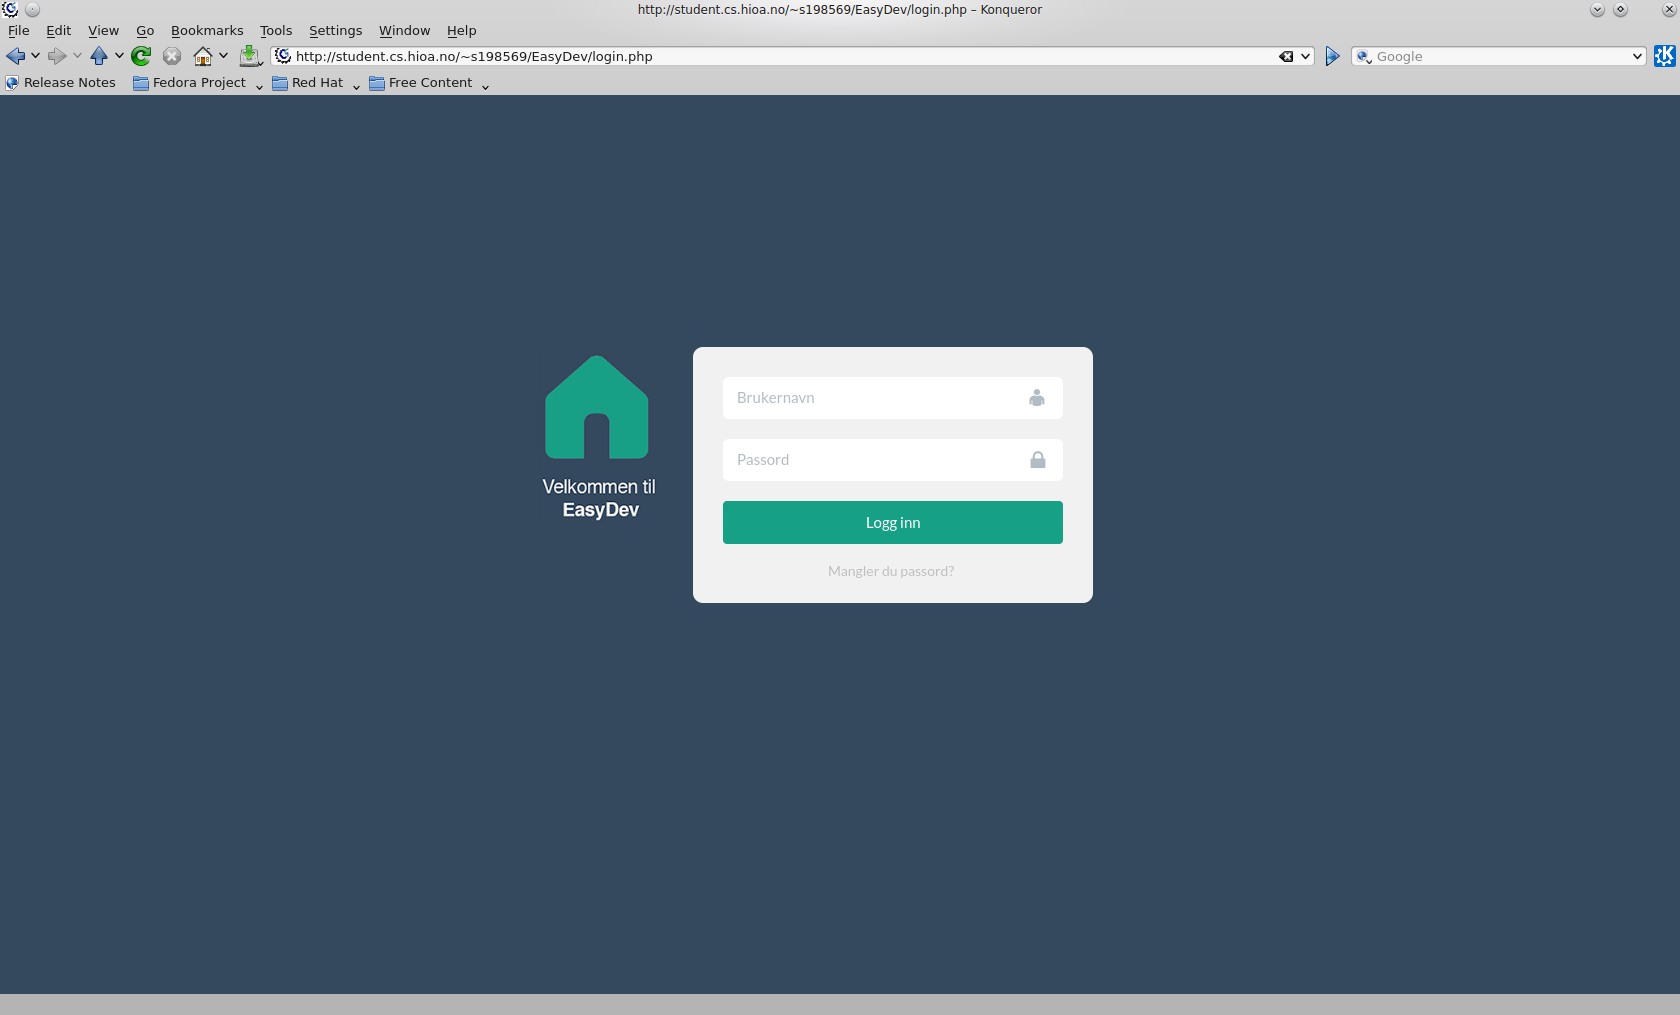
\includegraphics[width=\textwidth,height=\textheight,keepaspectratio]{./img/prosessdokumentasjon/hifi/login.png}
\caption[(Hi-fi) Påloggingsbilde]{Påloggingsbilde. I prtotypen er det mulig å logge seg på uten brukernavn eller passord. Etter dette påloggingsbilde blir brukeren forflyttet til fremside.}
\label{fig:loginhi}
\end{figure}

%KONFIGURASJON AV APACHE
\begin{figure}[ht]
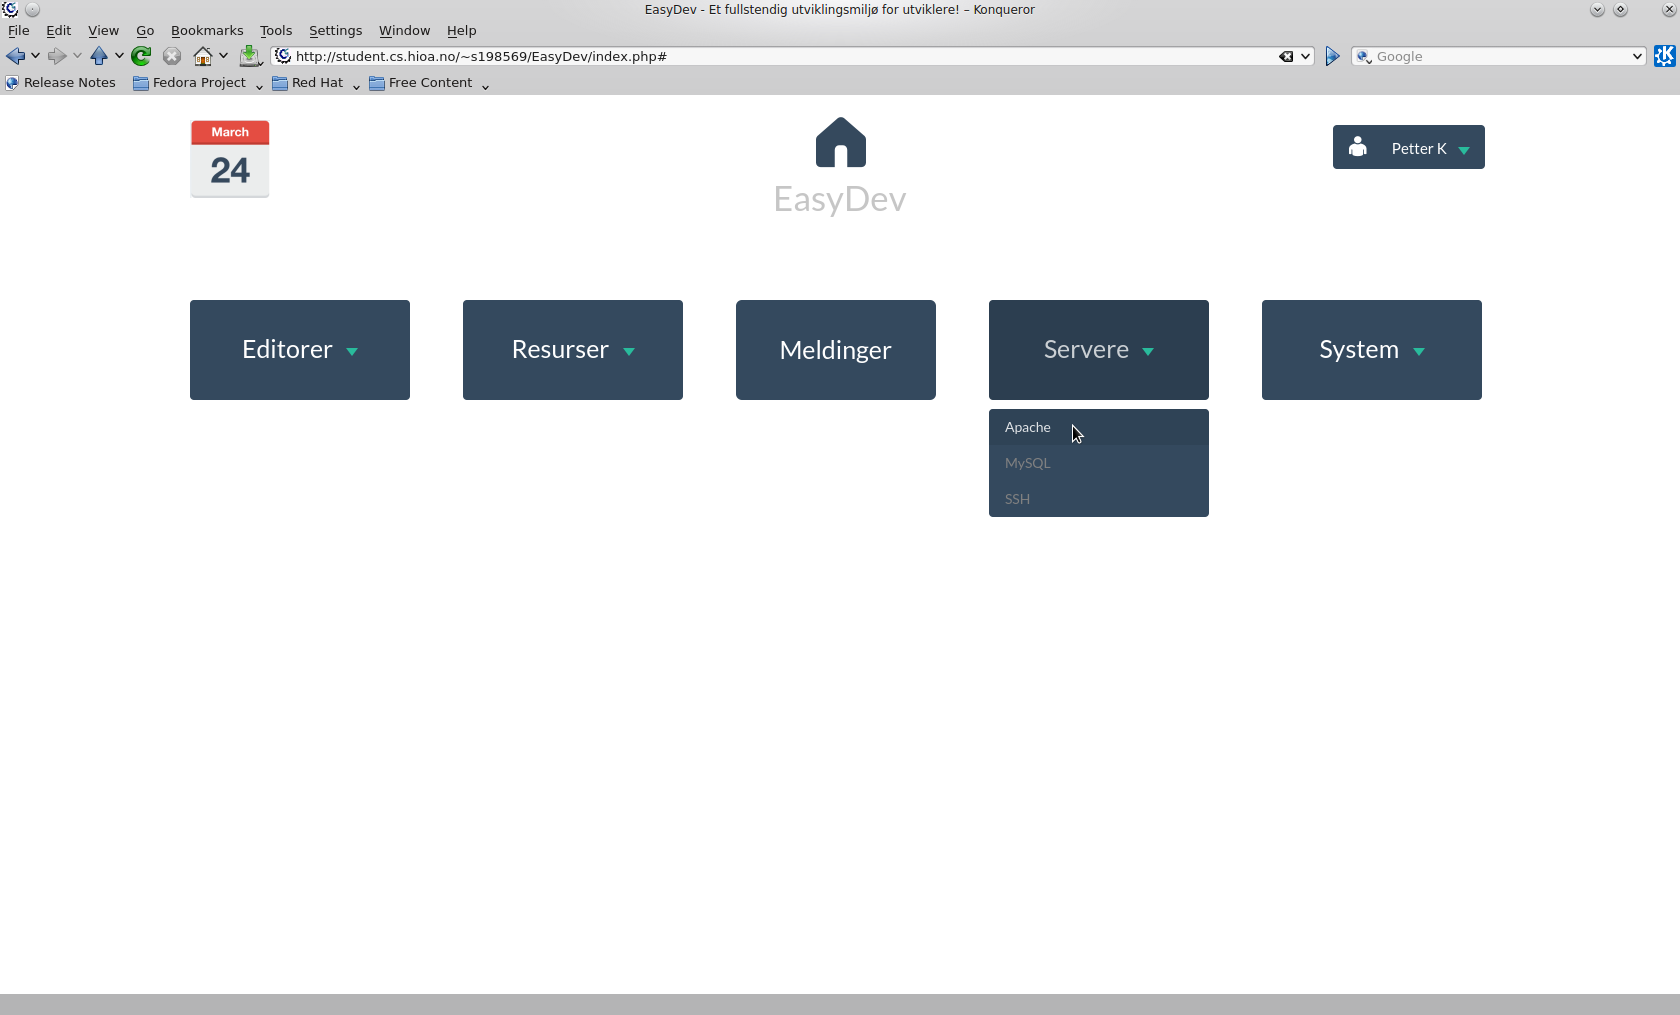
\includegraphics[width=\textwidth,height=\textheight,keepaspectratio]{./img/prosessdokumentasjon/hifi/a1.png}
\caption{(Hi-fi) Webserver: }
\label{fig:apachehi1}
\end{figure}

\begin{figure}[ht]
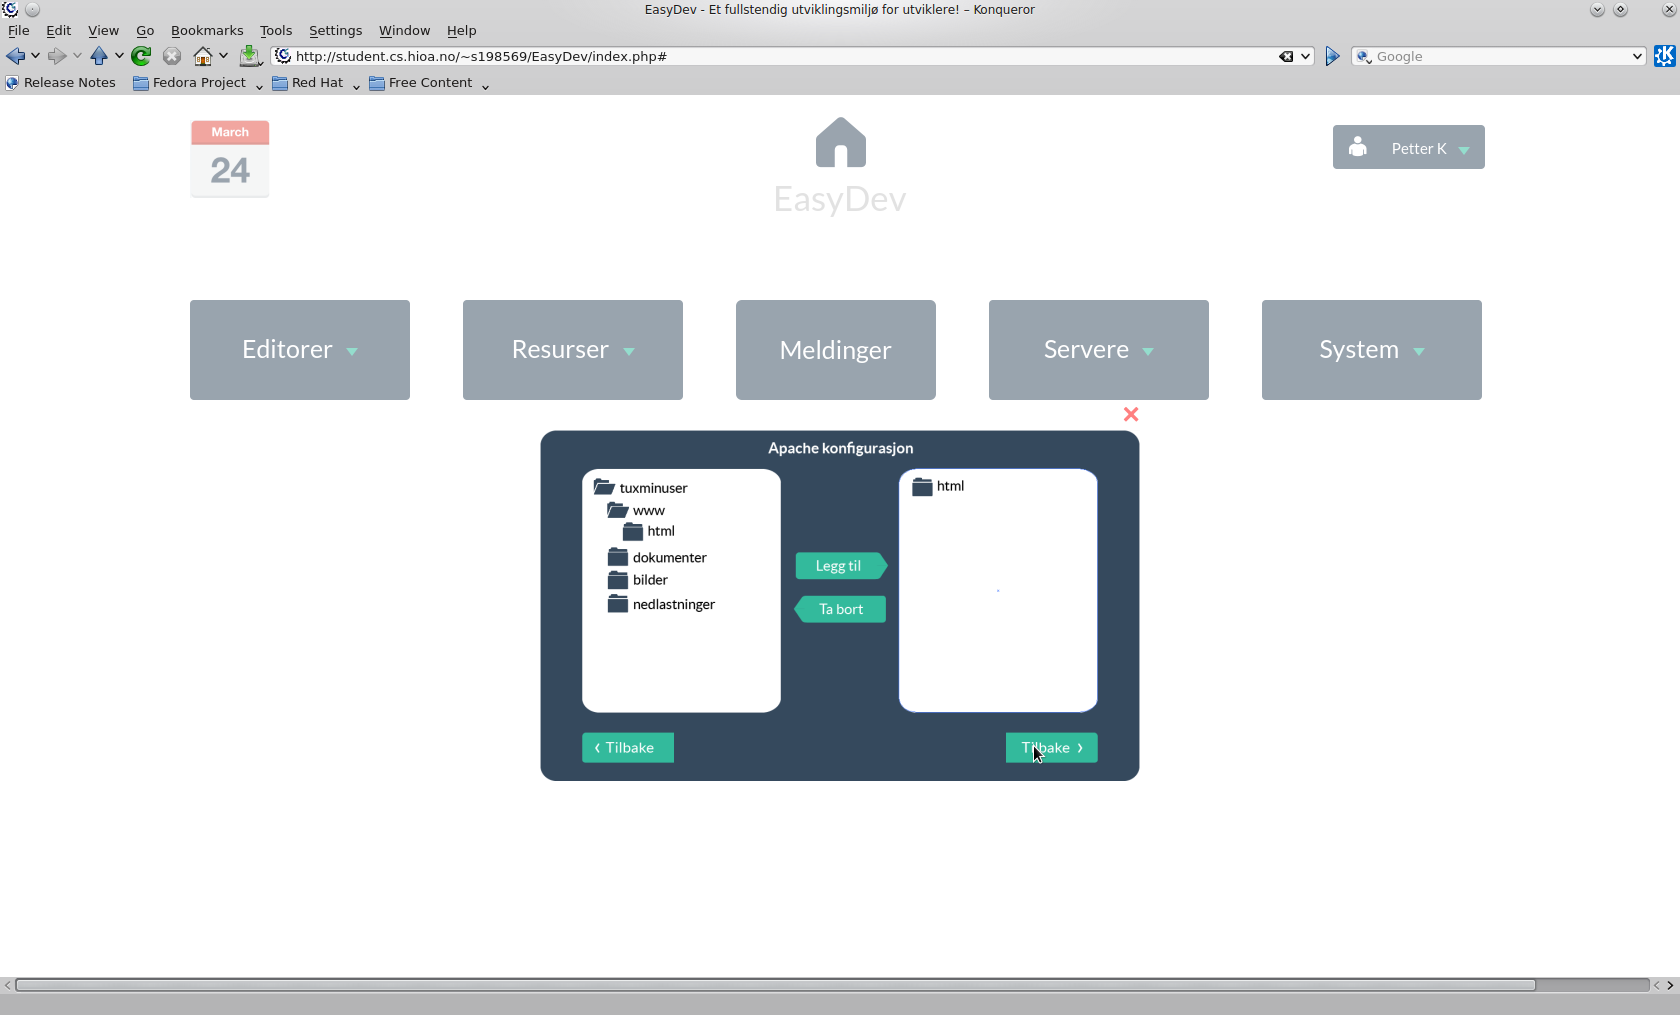
\includegraphics[width=\textwidth,height=\textheight,keepaspectratio]{./img/prosessdokumentasjon/hifi/a2.png}
\caption{(Hi-fi) Webserver: }
\label{fig:apachehi2}
\end{figure}

\begin{figure}[ht]
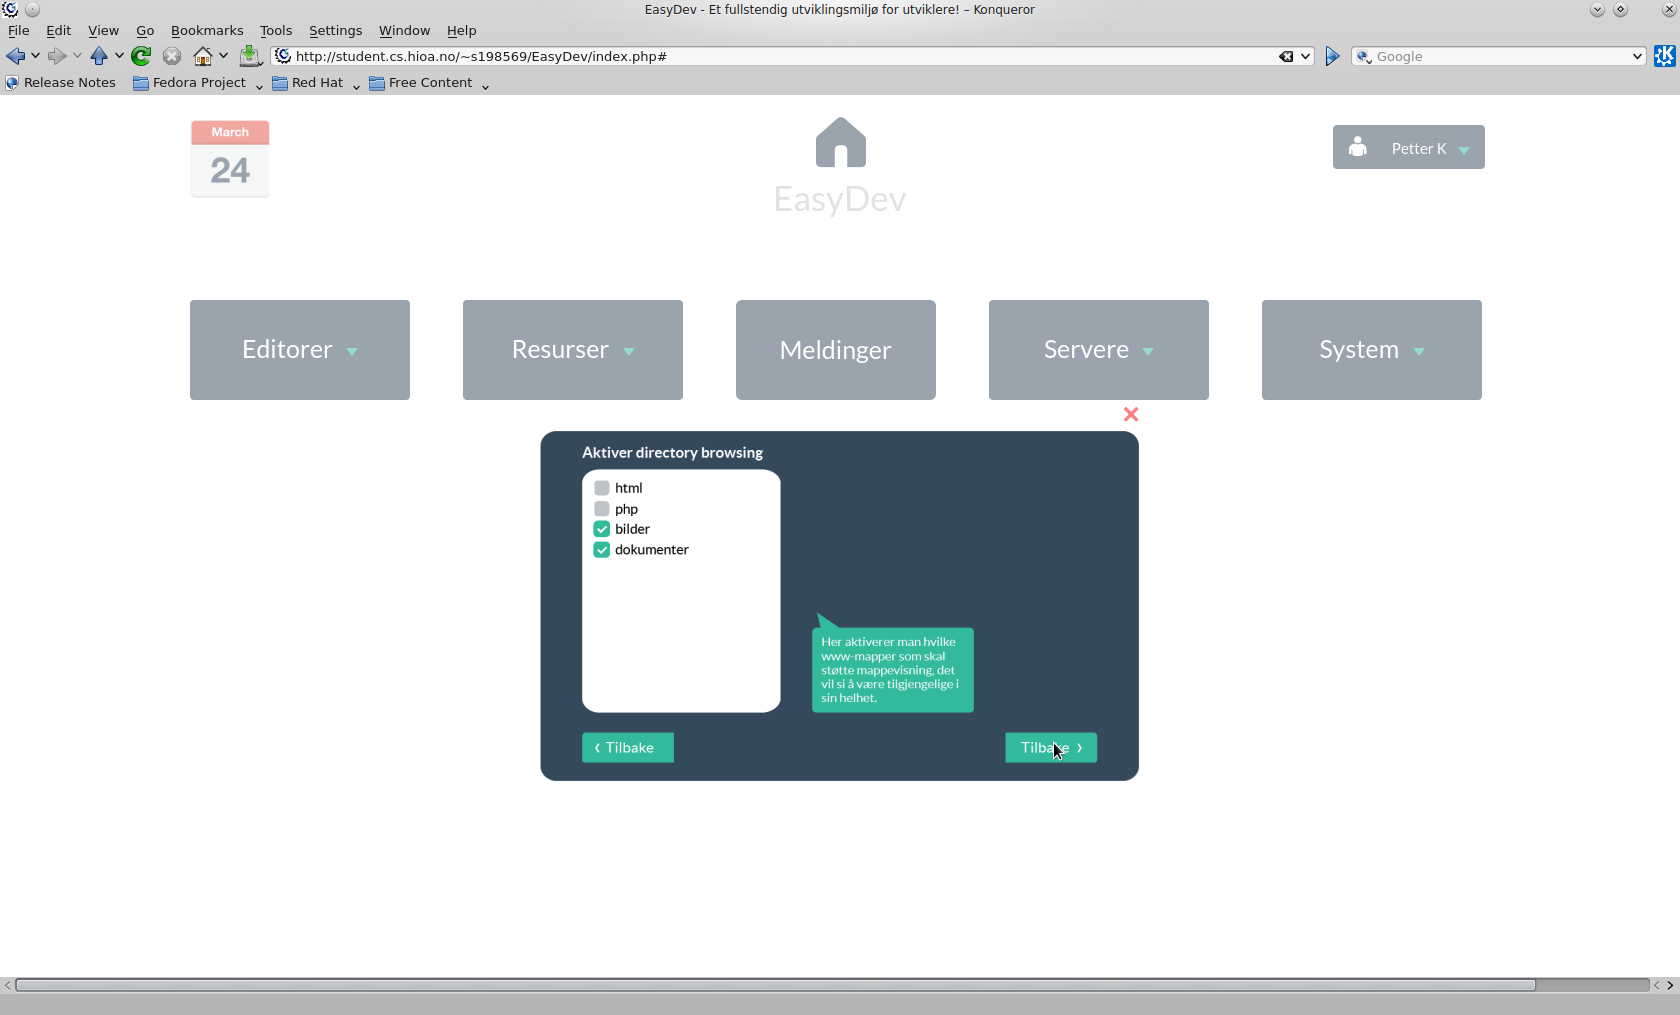
\includegraphics[width=\textwidth,height=\textheight,keepaspectratio]{./img/prosessdokumentasjon/hifi/a3.png}
\caption{(Hi-fi) Webserver: }
\label{fig:apachehi3}
\end{figure}

\begin{figure}[ht]
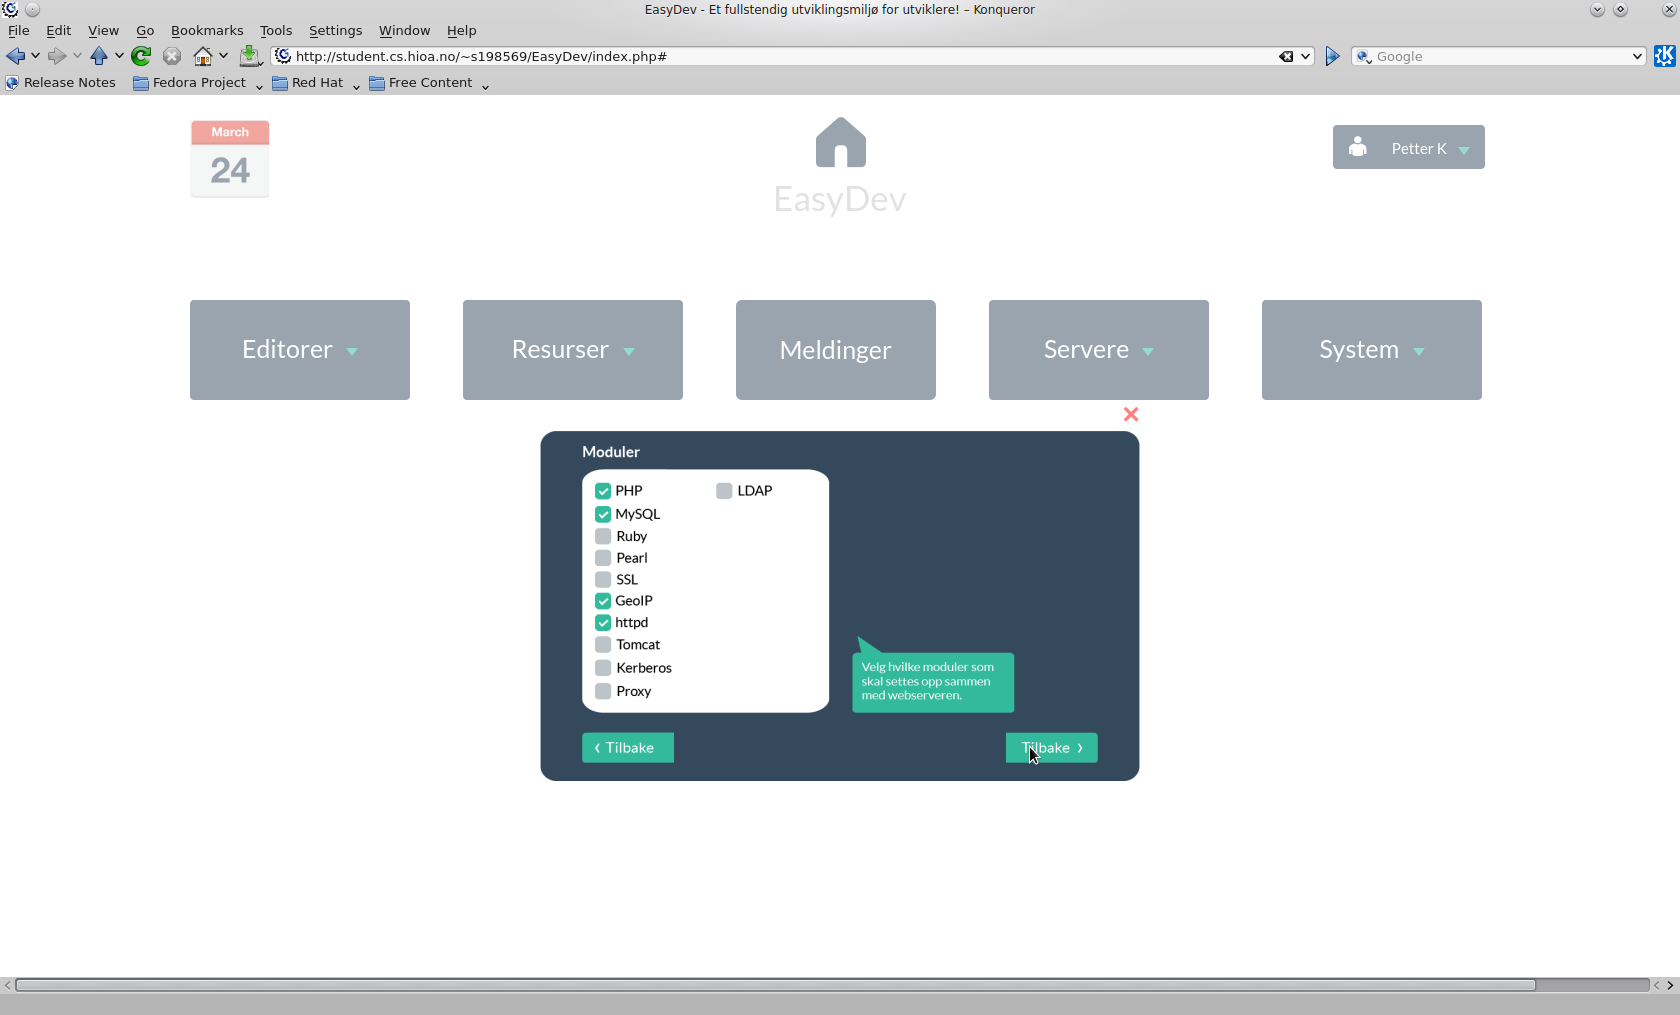
\includegraphics[width=\textwidth,height=\textheight,keepaspectratio]{./img/prosessdokumentasjon/hifi/a4.png}
\caption{(Hi-fi) Webserver: }
\label{fig:apachehi4}
\end{figure}

\begin{figure}[ht]
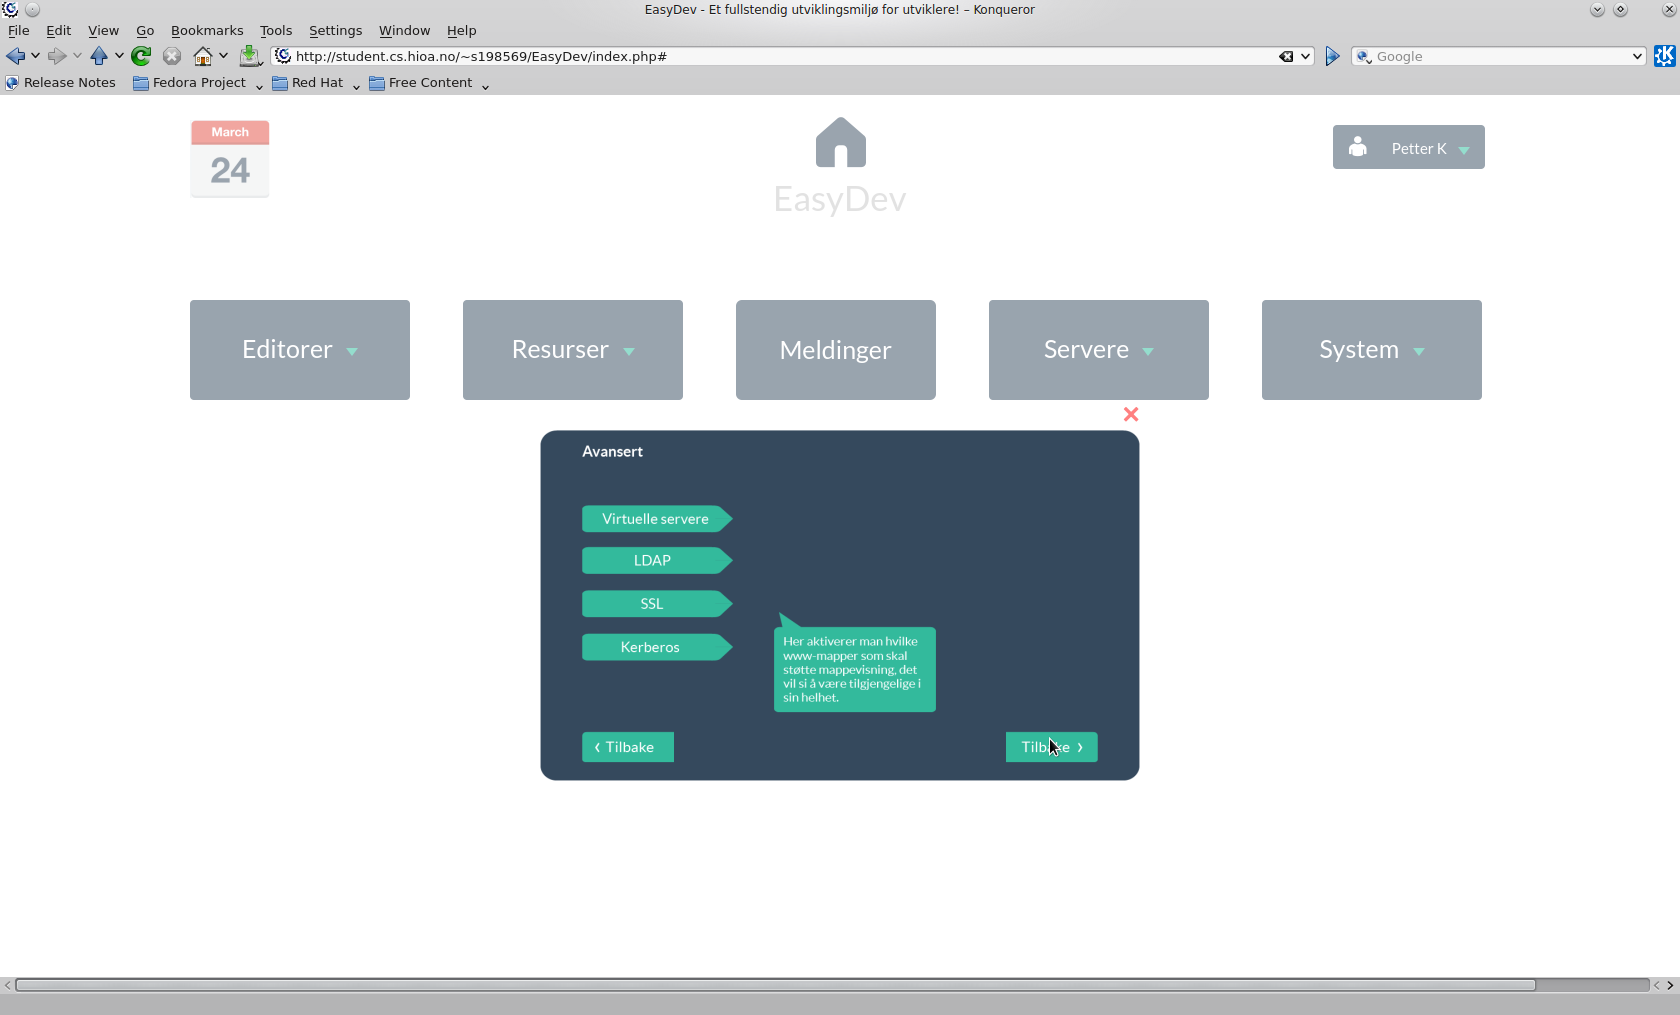
\includegraphics[width=\textwidth,height=\textheight,keepaspectratio]{./img/prosessdokumentasjon/hifi/a5.png}
\caption{(Hi-fi) Webserver:}
\label{fig:apachehi5}
\end{figure}

%KONFIGURASJON AV BRUKERE
\begin{figure}[ht]
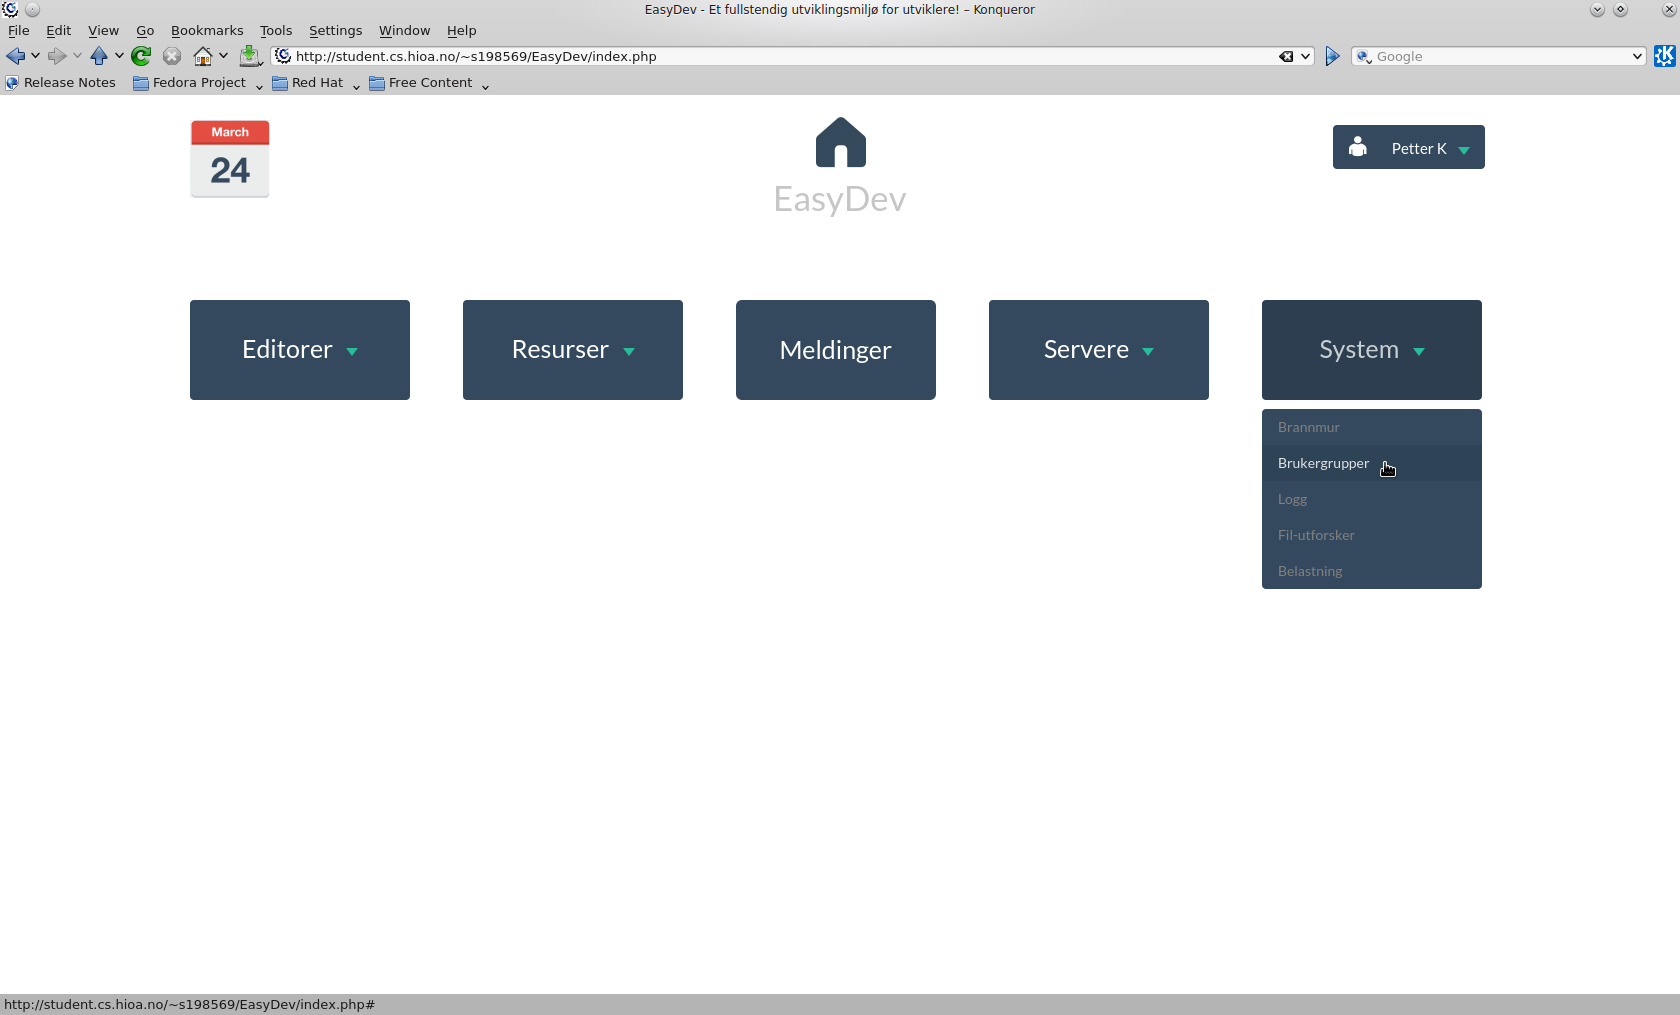
\includegraphics[width=\textwidth,height=\textheight,keepaspectratio]{./img/prosessdokumentasjon/hifi/b1.png}
\caption{Brukere: }
\label{fig:brukerehi1}
\end{figure}

\begin{figure}[ht]
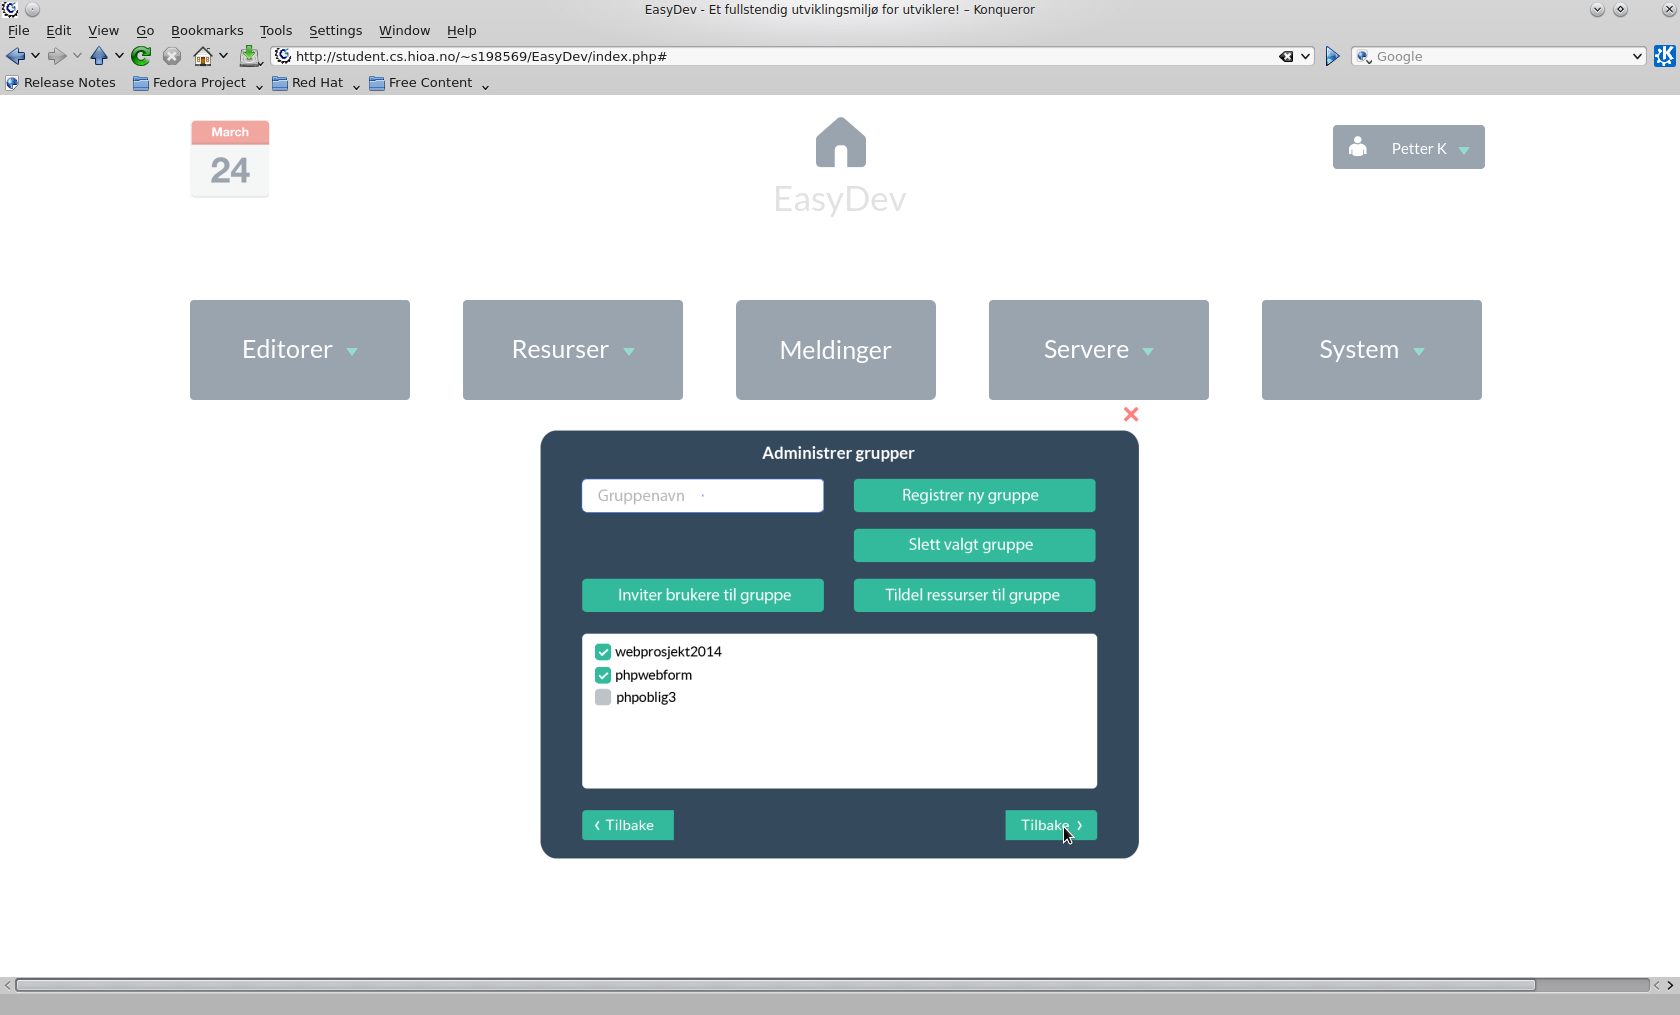
\includegraphics[width=\textwidth,height=\textheight,keepaspectratio]{./img/prosessdokumentasjon/hifi/b2.png}
\caption{Brukere: }
\label{fig:brukerehi2}
\end{figure}

\begin{figure}[ht]
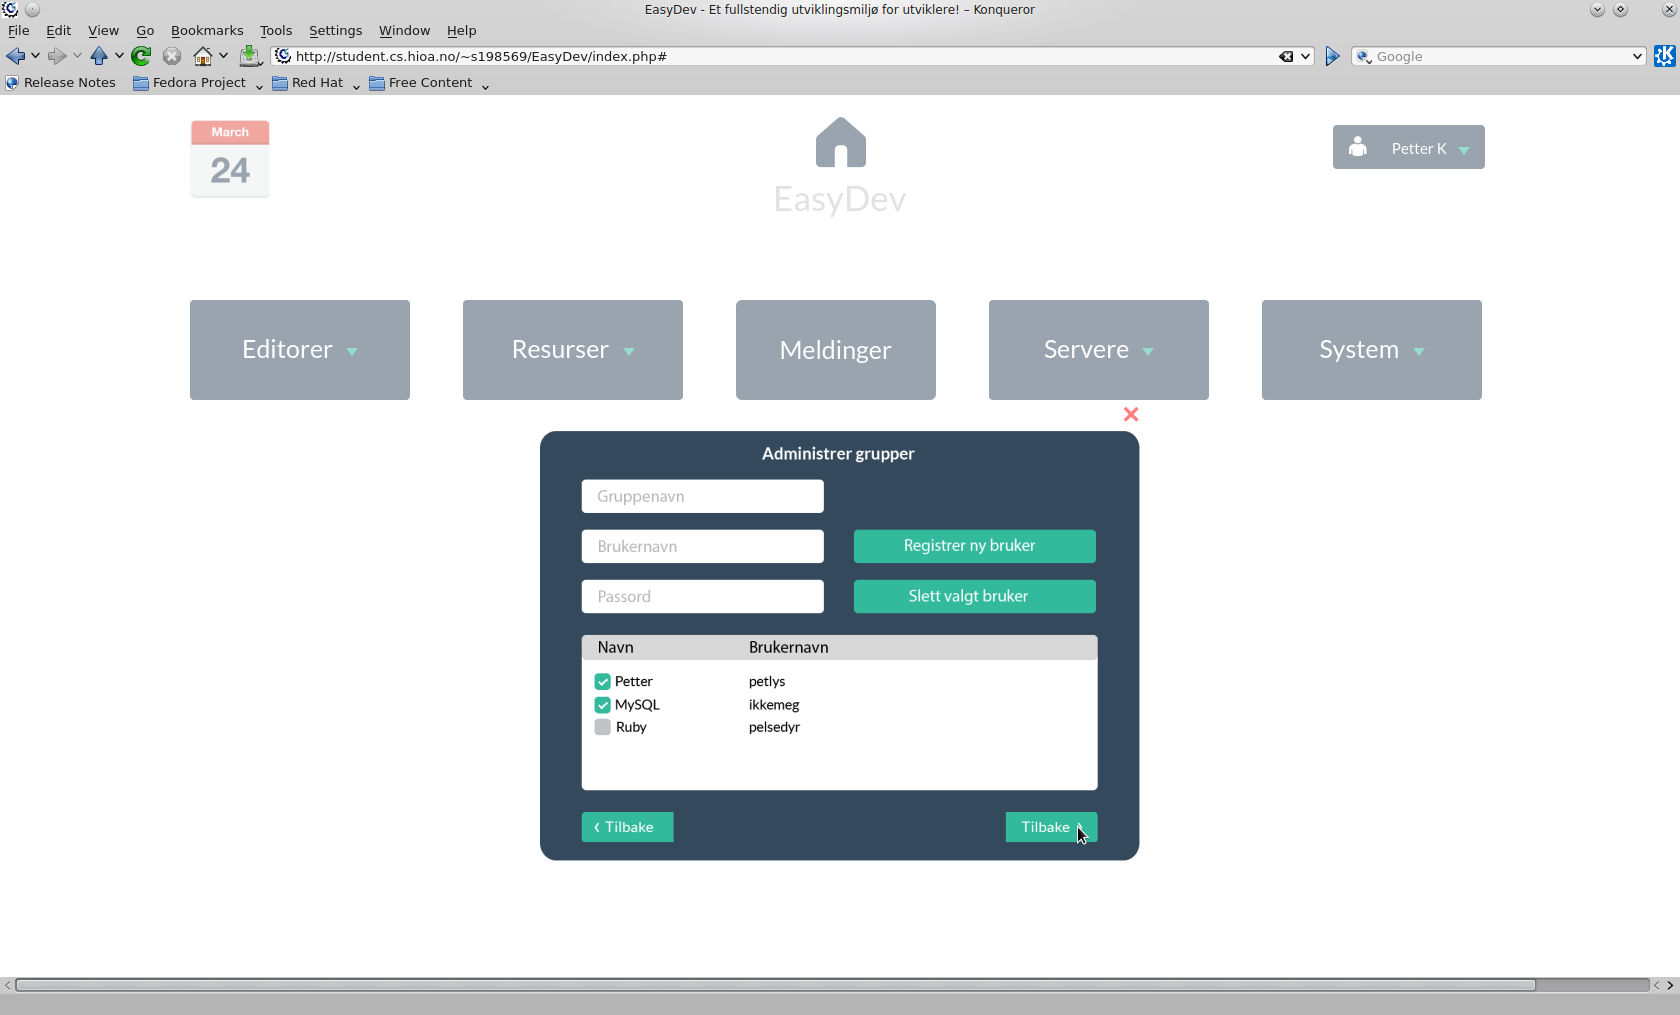
\includegraphics[width=\textwidth,height=\textheight,keepaspectratio]{./img/prosessdokumentasjon/hifi/b3.png}
\caption{Brukere: }
\label{fig:brukerehi3}
\end{figure}

\begin{figure}[ht]
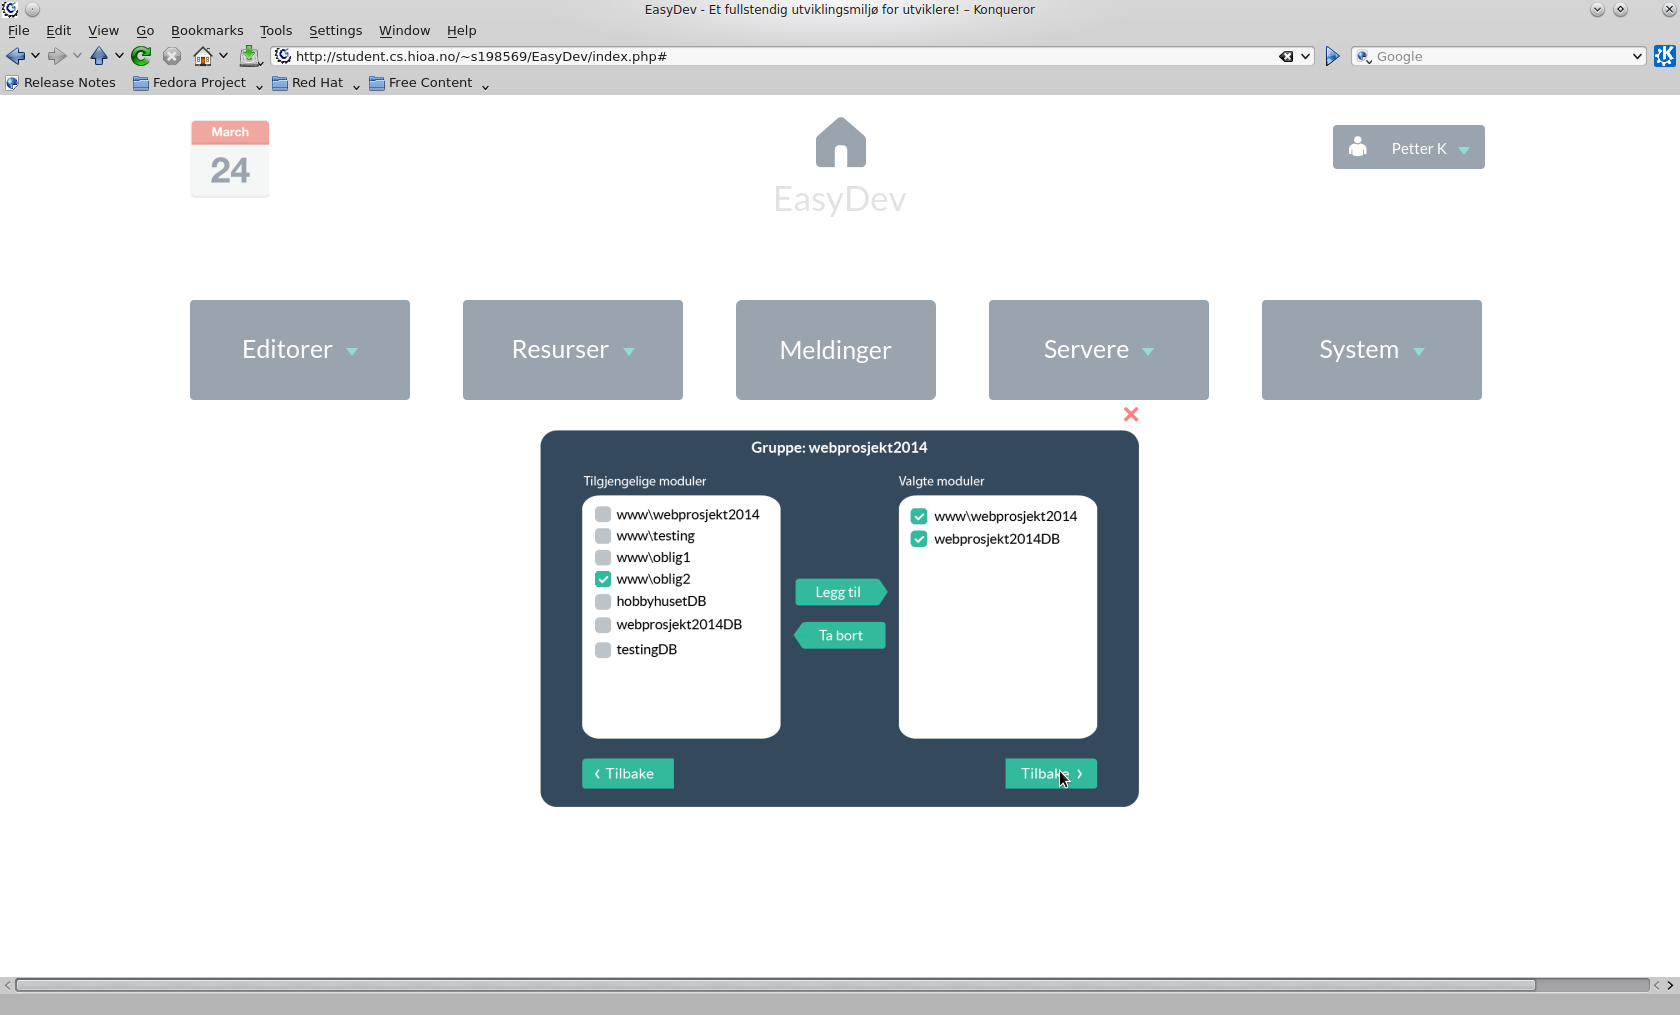
\includegraphics[width=\textwidth,height=\textheight,keepaspectratio]{./img/prosessdokumentasjon/hifi/b4.png}
\caption{Brukere: }
\label{fig:brukerehi4}
\end{figure}